\documentclass{article}
\usepackage[utf8]{inputenc}
\usepackage{float}
\usepackage{amssymb}
\usepackage{amsmath}
\usepackage{algorithm}
\usepackage{import}
\usepackage{algcompatible}
\usepackage{algpseudocode}
\usepackage{parskip}
\usepackage{minted}
\usepackage{commath}
\usepackage{tikz}
\usepackage{hyperref}

\usepackage[margin=2.2cm]{geometry}


\title{Theory Assignment-5: ADA Winter-2024}
\author{Rachit Arora (2022384) \and Mahi Mann (2022272)}

\date{}
\begin{document}
\floatplacement{figure}{H}

\maketitle

\section{Assumptions}

\begin{itemize}
    \item A box $B_2$ can only be placed inside a box $B_1$ if dimensions of $B_2$ can be rearranged to be \textbf{strictly smaller} than dimensions of $B_1$. If not, some trivial minor changes can be made to the implementation. 
\end{itemize}

\section{Formulation as a Network Flow problem}

Let there be $n$ boxes $B_1, B_2, \cdots, B_n$. with dimensions $d_1 = (x_1, y_1, z_1), d_2 = (x_2, y_2, z_2), \cdots, d_n$.

We want to minimise $k = \text{number of visible boxes}$. 

\textbf{$k$ can also be expressed as $n - v$ where $v$ is the number of invisible boxes.}

Thus, we have an equivalent problem of \textbf{maximising $v$, the number of invisible boxes.} 

\section{Why Max Flow corresponds to answer}


\section{Complexity Analysis (Using Ford-Fulkerson's Algorithm)}

To solve this Max-Flow problem, we are running the Ford-Fulkerson Algorithm on our auxiliary bipartite graph construction $G = (V, E)$ where $\abs{V} = O(n)$ and $\abs{E} = O(n^2)$ (see Proof of Correctness section for cardinality of $E$).

As will be proved shortly, the maximum possible flow in this graph is also the maximum number of invisible boxes, which is $value(flow) = n-1 = O(n)$. 

Ford-Fulkerson's Algorithm runs in $O(value(flow)(\abs{V} + \abs{E}))$ time, \textbf{therefore our algorithm runs in}

    \begin{center}
    \begin{align*}
        O\left(value(flow)\left( \abs{V} + \abs{E} \right) \right) \\
        = O(value(flow)) O(\abs{V} + \abs{E}) \\
        = O(n) O(n + n^2) \\
        = O(n) O(n^2) \\
        = O(n^3) 
    \end{align*}
    \end{center}

$O(n^3)$ \textbf{time where $n$ is the number of boxes.}


\section{Proof of Correctness}


\section*{Addendum 1: C++ implementation}


\section*{Addendum 2: Sample Tests}

% \subsection{Test 1}
% \subsubsection*{Input}
% \inputminted{sh}{./in1}
% \subsubsection*{Graph description}
% \begin{figure}
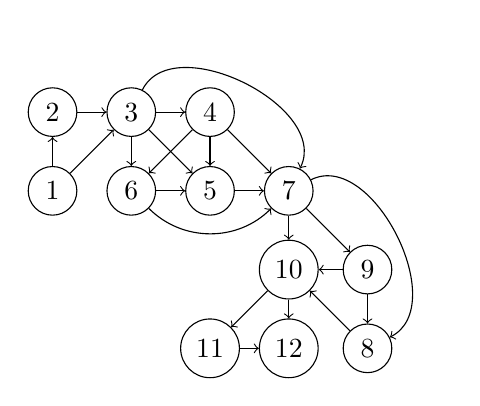
\begin{tikzpicture}[->, nodes={draw, circle}, scale=0.5]

  \node (1) {1};
  \node (2) [above of=1] {2};
  \node (3) [right of=2] {3};
  \node (4) [right of=3] {4};
  \node (6) [below of=3] {6};
  \node (5) [right of=6] {5};
  \node (7) [right of=5] {7};
  \node (10) [below of=7] {10};
  \node (9) [right of=10] {9};
  \node (8) [below of=9] {8};
  \node (12) [left of=8] {12};
  \node (11) [left of=12] {11};

  \path (1) edge (2);
  \path (1) edge (3);
  \path (2) edge (3);
  \path (3) edge (4);
  \path (4) edge (5);
  \path (3) edge (6);
  \path (3) edge (5);
  \path (4) edge (6);
  \path (6) edge (5);
  \path (4) edge (7);
    \path (3) edge [bend left=90](7);
  \path (5) edge (7);
  \path (6) edge [bend right = 45](7);
    \path (7) edge [bend left=90](8);
  \path (7) edge (9);
  \path (7) edge (10);
  \path (9) edge (8);
  \path (9) edge (10);
  \path (8) edge (10);
  \path (10) edge (11);
  \path (10) edge (12);
  \path (11) edge (12);
\end{tikzpicture}
\end{figure}

% \subsubsection*{Output}
% \inputminted{sh}{./out1}
% \subsubsection*{Output illustration}
% \begin{figure}
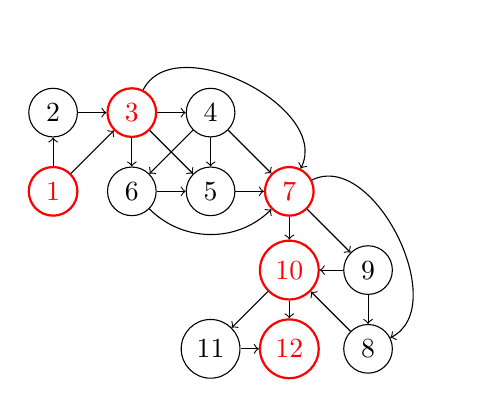
\begin{tikzpicture}[->, nodes={draw, circle}, scale=0.5]

  \node (1) [red, thick]{1};
  \node (2) [above of=1] {2};
  \node (3) [red, thick, right of=2] {3};
  \node (4) [right of=3] {4};
  \node (6) [below of=3] {6};
  \node (5) [right of=6] {5};
  \node (7) [red, thick][right of=5] {7};
  \node (10) [red, thick, below of=7] {10};
  \node (9) [right of=10] {9};
  \node (8) [below of=9] {8};
  \node (12) [red, thick][left of=8] {12};
  \node (11) [left of=12] {11};

  \path (1) edge (2);
  \path (1) edge (3);
  \path (2) edge (3);
  \path (3) edge (4);
  \path (4) edge (5);
  \path (3) edge (6);
  \path (3) edge (5);
  \path (4) edge (6);
  \path (6) edge (5);
  \path (4) edge (7);
    \path (3) edge [bend left=90](7);
  \path (5) edge (7);
  \path (6) edge [bend right = 45](7);
    \path (7) edge [bend left=90](8);
  \path (7) edge (9);
  \path (7) edge (10);
  \path (9) edge (8);
  \path (9) edge (10);
  \path (8) edge (10);
  \path (10) edge (11);
  \path (10) edge (12);
  \path (11) edge (12);

\end{tikzpicture}
\end{figure}



\section*{Addendum 3: People discussed with}

Swapnil Panigrahi, Sahil Gupta and Yash Bhardwaj.

\vspace*{\fill}
\begin{center}
    $\square \square \square \square \square$
    \\
    Thank you.
\end{center}
\vspace*{\fill}

\end{document}
